\documentclass[a4paper, 12pt]{article}

\usepackage{graphicx}
\usepackage[font=small, labelfont=bf, labelsep=colon]{caption}
\usepackage{amsmath, amssymb}
\usepackage{float}
\usepackage{textcomp}
\usepackage{siunitx}
\usepackage[dvipsnames]{xcolor}
\usepackage{titling} % To allow to use \matitle more than once
\usepackage{ctable}
\usepackage{multirow}
\usepackage[flushmargin, bottom]{footmisc} 
\usepackage{hyperref}

\hypersetup{
colorlinks = true,
linkcolor = {blue!80!black}
}

\graphicspath{{../../../Pictures/}}

%%%%%%%%%%%%%%%%%%%%%%%%%%%%%%%%%%%%%%%%%%%%%%%%%%%%%%%
% Layout parameters 
\setlength{\parindent}{0em}
\setlength{\parskip}{2ex}
\linespread{1.2}

\renewcommand{\floatpagefraction}{.99} % Minimum fraction of floats, in a page that has only floats. Only figures taking up more than that will get their own page. Default 0.5
\renewcommand{\topfraction}{0.99}  % Maximum fraction of page for floats at top. I.e.: floats taking up more than this will have no text below. Default: 0.7.
\renewcommand{\textfraction}{0.01} % Minimum fraction of page that must have text (otherwise, the page will only have float). Default: 0.2 

\addtolength{\textwidth}{2cm}
\addtolength{\hoffset}{-1cm}
\setlength{\topmargin}{-1cm}
\addtolength{\textheight}{1cm}

\setlength{\skip\footins}{6mm} % space between end of text and horizontal line of footnote
\setlength{\footnotesep}{5mm} % space between footnote line and first entry, and between consecutive entries of footnote



%%%%%%%%%%%%%%%%%%%%%%%%%%%%%%%%%%%%%%%%%%%%%%%%%%

%%%%%%%%%%%%%%%%%%%%%%%%
%%%%% NEW COMMANDS
%%%%%%%%%%%%%%%%%%%%%%%%

% Text commands
\newcommand{\spc}{1ex}
\newcommand{\eg}{\textit{e.g.}}
\newcommand{\ie}{\textit{i.e.}}

% Maths Commands
\newcommand{\R}{\mathbb{R}}
\newcommand{\bd}[1]{\boldsymbol{#1}}
\newcommand{\x}{\bd x}
\newcommand{\A}{{_{[A]}}}
\newcommand{\xA}{\bd{x^\A}}
\newcommand{\eps}{\varepsilon}
\newcommand{\Nr}{N_\text{regr}}
\newcommand{\E}{\mathbb{E}}
\newcommand{\Var}{\text{Var}}

\newcommand{\D}{\mathcal{D}}


\newcommand{\ya}{y^{(\alpha)}}
\newcommand{\yb}{y^{(\beta)}}
\newcommand{\ta}{\bd{\widetilde \alpha}}
\newcommand{\tb}{\bd{\widetilde \beta}}



%%%%%%%%%%%%%%%%%%%%%%%%%%%%%%%%%%%%%%%%%%%%%%%%%%%%%

\title{New Emulators for Monthly Gas Consumption}

\author{}
\date{}

\begin{document}

\maketitle
\vspace{-9ex}


This document is a concise summary of the construction and validation of the monthly gas consumption emulators. 
The 1000 design runs are divided into a group of 800 used for training, and a group of 200 used for validation.
For reference, \autoref{Table_Var_names} lists the meaning and range of the 8 inputs which are varied from one simulation to the other.

\begin{table}
 \centering
 \renewcommand{\arraystretch}{1.4}
 \newcommand{\colsep}{4ex}
 \caption{Meaning and range of the eight parameters varied among the $n$ simulations of this work. {\it \footnotesize(Mohammad may provide more appropriate descriptions for the middle column.)}}
 \begin{tabular}{c<{\hspace{\colsep}}  c<{\hspace{\colsep}}  c}
\specialrule{.1em}{0em}{0.1em} 
 \textbf{Short Name} &  \textbf{Physical Meaning} & \textbf{Range} \\
 \specialrule{.05em}{.1em}{0.1em} 
 \specialrule{.05em}{0em}{0.2em} 
  $V_1$   &  Heating Setpoint               &  $[17.5, 20.5]$ $\si{\celsius}$        \\
  $V_2$   &  Boiler Efficiency              &  $[0.6, 0.75]$                         \\
  $V_3$   &  External wall thickness        &  $[4, 6.3]$ cm                         \\
  $V_4$   &  Roof quilt thickness           &  $[15, 21]$ cm                         \\
  $V_5$   &  Floor insulation thickness     &  $[4.5, 5.5]$ cm                       \\
  $V_6$   &  Infiltration rate              &  $[0.2, 0.95]$ ac/h                    \\
  $V_7$   &  DHW Consumption                &  $[6.15, 22] \!\times\! 10^{-6}$ litre/day \\
  $V_8$   &  Cooking                        &  $[1.05, 6.3]$ W/m$^2$                 \\
 \specialrule{.1em}{0.2em}{1em} 
 \end{tabular}
\label{Table_Var_names}
\end{table}

\section{Emulators' Training}
In order to emulate the monthly gas consumption, the range of each of the eight input variables $V_1, \dots, V_8$ has been linearly rescaled into $[-1,1]$.
Given the outputs $y_i$ of the 800 training runs for a month, 
I have first built a linear regression model of $y_i$ as a function of (some of the) linear, quadratic and interaction terms of the $V_i$.
Hence, I have built an emulator of the linear regression residuals. Details of the two steps follow.

\subsubsection*{Linear Regression}
Let $\mathcal{R}$ be the set of all linear, quadratic and interaction terms of the 8 inputs $V_1, \dots, V_8$, all mutually orthogonal.
As it turns out, for all months, the set of the ``best'' 10 regressors in $\mathcal{R}$ (the set maximising the adjusted $R^2$) explains the data extremely well, 
with an adj-$R^2$ of about 0.999 in all cases. Given the excellent result, and to use an approach which is uniform among months and simple to explain,  
for each month I have built a linear regression model by selecting the best 10 regressors according to the above criterion. 
\emph{(previously, for May, I was using some 3rd-order terms to improve the linear model. Probably not worth it)}

\autoref{Table_Regressors} shows which 10 regressors have been selected for each month, the adjusted $R^2$ of the associated linear model, and the variance of the residuals.

\begin{table}
 \centering
 \renewcommand{\arraystretch}{1.4}
 \newcommand{\colsep}{3ex}
 \caption{For each of the nine months considered, from left to right: the set of covariates used to build the linear regression model, the adjusted $R^2$ of the model, the variance of the residuals.
 In the second column, the ``$\ast$'' symbol is used as shorthand notation to denote all linear and interaction terms, \eg\ $\,a \ast b \ast c = \{ a, b, c , ab, ac, bc \}$.}
 \begin{tabular}{c<{\hspace{\colsep}}  c<{\hspace{\colsep}}  c<{\hspace{\colsep}} c}
\specialrule{.1em}{0em}{0.1em} 
 \textbf{Month} &  \textbf{Regressors} & \textbf{Adj.~$R^2$} & \textbf{Resid.~Var.~$\sigma^2$}\\
 \specialrule{.05em}{.1em}{0.1em} 
 \specialrule{.05em}{0em}{0.2em} 
  Jan  &  $V_1 \!\ast\! V_2 \!\ast\! V_6, \,V_3,\, V_4,\,{V_2}^2,\, {V_6}^2$   & 0.9998   & 84.86\\
  Feb  &  $V_1 \!\ast\! V_2 \!\ast\! V_6, \,V_3,\, V_4,\,{V_2}^2,\, {V_6}^2$   & 0.9998  &  50.63\\
  Mar  &  $V_1 \!\ast\! V_2 \!\ast\! V_6, \,V_3,\, V_4,\,{V_2}^2,\, {V_6}^2$   & 0.9997  &  49.14\\
  Apr  &  $V_1 \!\ast\! V_2 \!\ast\! V_6, \,V_3,\, V_4,\,{V_2}^2,\, {V_6}^2$   & 0.9998  &  49.58\\  
  May  &  $V_1 \!\ast\! V_2 \!\ast\! V_6, \,V_3,\, V_8,\,{V_1}^2,\, {V_6}^2$   & 0.9989  & 206.70\\
  Sep  &  $V_1 \!\ast\! V_2 \!\ast\! V_6, \,V_3,\, V_4,\, V_8,\, {V_6}^2$         & 0.9995  &  0.88\\
  Oct  &  $V_1 \!\ast\! V_2 \!\ast\! V_6, \,V_3,\, V_4,\, V_8,\, {V_6}^2$         & 0.9996  &  23.20\\
  Nov  &  $V_1 \!\ast\! V_2 \!\ast\! V_6, \,V_3,\, V_4,\,{V_2}^2,\, {V_6}^2$   & 0.9998 &  57.22\\
  Dec  &  $V_1 \!\ast\! V_2 \!\ast\! V_6, \,V_3,\, V_4,\,{V_2}^2,\, {V_6}^2$   & 0.9998  &  67.65\\
 \specialrule{.1em}{0.2em}{1em} 
 \end{tabular}
\label{Table_Regressors}
\end{table}


\subsubsection*{Bayes Linear Emulators of Residuals}
In order to build an emulator of the residuals, choices about the following are to be made: active inputs, correlation lengths, prior emulator variance and nugget variance.

To choose these, for each month, I have followed the general procedure which I highlight below. However, some of the choices necessarily follow from a considerable and necessarily subjective work of ``try $\rightleftarrows$ validate, then make a decision'', rather than from the ``blind'' application of a single rule. Hope this still sounds good for the paper, one we should validation plots? (details in the next section)

\begin{itemize}
\item {\bf Active Inputs}: To identify which inputs were significant in explaining the residuals, I have looked at the best selection of second- (and sometimes third-) order terms in a linear model. 
Terms which would appear alone with a significant $t$-value ($t>8$) would generally be included as an active input, while the inclusion of terms appearing only in interaction with other terms, or with a low $t$-value would be considered case by case, with a process of trial and error.
\item {\bf Correlation lengths}: Once the active inputs have been chosen, for simplicity I have used the same correlation length for all of them. The correlation length has been chosen by a repeated trial-and-validation procedure, adjusted to the number of active inputs used (if more active inputs are used, higher correlation lengths are required to maintain a similar level of correlation across the input space).
\item {\bf Prior Variances}: The cumulative prior variance (the one of the second-order stochastic process over which we make specifications, and the one of the ``nugget'' process) has been imposed to be the variance of the residuals which are being fitted. This overall variance has been split into the two components in the proportions of $95\%$ and $5\%$ respectively.
\end{itemize}

\autoref{Table_Emulator_Specifications} shows the choices of the above quantities for the nine months of interest.
\autoref{Fig_Correlation} instead gives an idea of the level of correlation across the input space induced by the above choices. Specifically, called $P$ the point at the centre of the hypercube with edges $[-1,1]$, the figure shows histograms of the correlation between the point $P$ and the 1000 design points.



\begin{table}
 \centering
 \renewcommand{\arraystretch}{1.4}
 \newcommand{\colsep}{3ex}
 \caption{For each of the nine months considered, the table below shows which active inputs have been chosen and the value of the correlation length (same for all active inputs).}
 \begin{tabular}{c<{\hspace{\colsep}}  c<{\hspace{\colsep}}  c<{\hspace{\colsep}} c}
\specialrule{.1em}{0em}{0.1em} 
 \textbf{Month} &  \textbf{Active Inputs} & \textbf{Corr.~Length}\\
 \specialrule{.05em}{.1em}{0.1em} 
 \specialrule{.05em}{0em}{0.2em} 
  Jan  &  $V_1, \,V_2, \,V_3, \,V_6, \,V_8$               &  0.8\\
  Feb  &  $V_1, \,V_2, \,V_3, \,V_7, \,V_8$               &  0.5\\
  Mar  &  $V_1, \,V_2, \,V_3, \,V_6, \,V_7, \,V_8$   &  1.2\\
  Apr  &  $V_1, \,V_2, \,V_3, \,V_6, \,V_8$              &  0.7\\  
  May  &  $V_1, \,V_2, \,V_3, \,V_4, \,V_6, \,V_8$  &  1.2\\
  Sep  &  $V_1, \,V_2, \,V_3, \,V_6, \,V_7, \,V_8$   &  1.0\\
  Oct  &  $V_1, \,V_2, \,V_3, \,V_6, \,V_7, \,V_8$   &  1.2\\
  Nov  & $V_1, \,V_2, \,V_3, \,V_6, \,V_7, \,V_8$   & 1.2\\
  Dec  &  $V_1, \,V_2, \,V_3, \,V_6, \,V_7, \,V_8$  & 1.3\\
 \specialrule{.1em}{0.2em}{1em} 
 \end{tabular}
\label{Table_Emulator_Specifications}
\end{table}


\newcommand{\scale}{12.7em}
\begin{figure}
\centering
 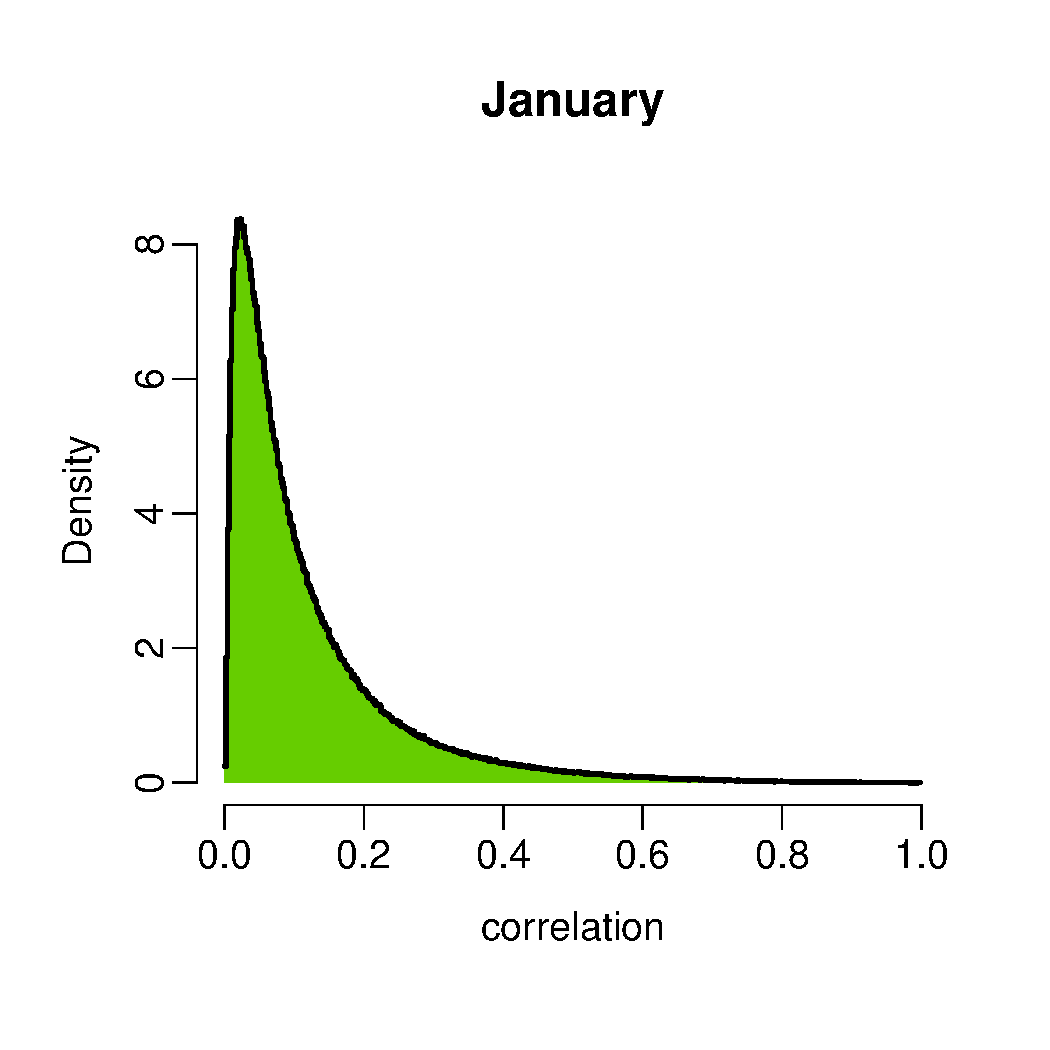
\includegraphics[width=\scale]{Validation_Plots/Correlation/Correlation_01_Jan}\hspace{-1ex}
 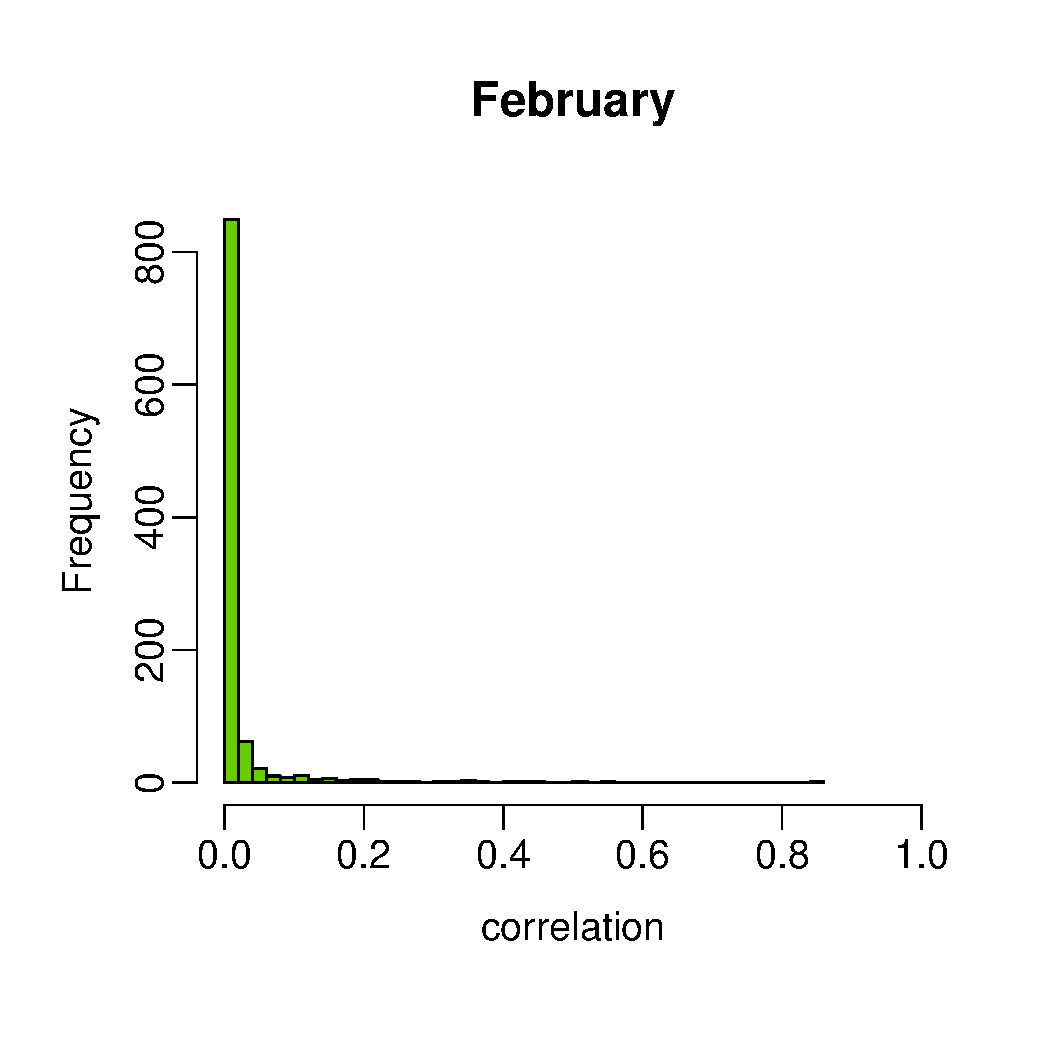
\includegraphics[width=\scale]{Validation_Plots/Correlation/Correlation_02_Feb}\hspace{-1ex}
 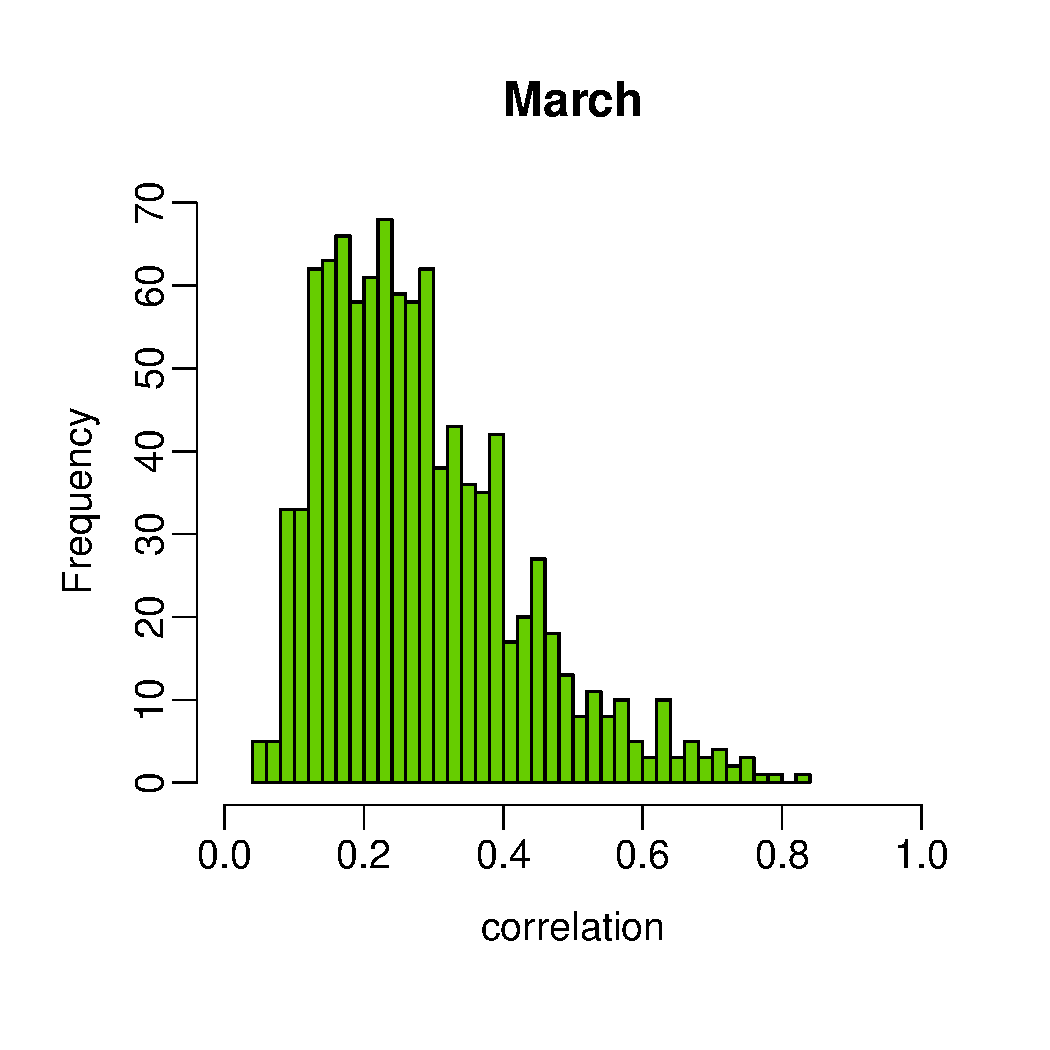
\includegraphics[width=\scale]{Validation_Plots/Correlation/Correlation_03_Mar}\\[-3ex]
 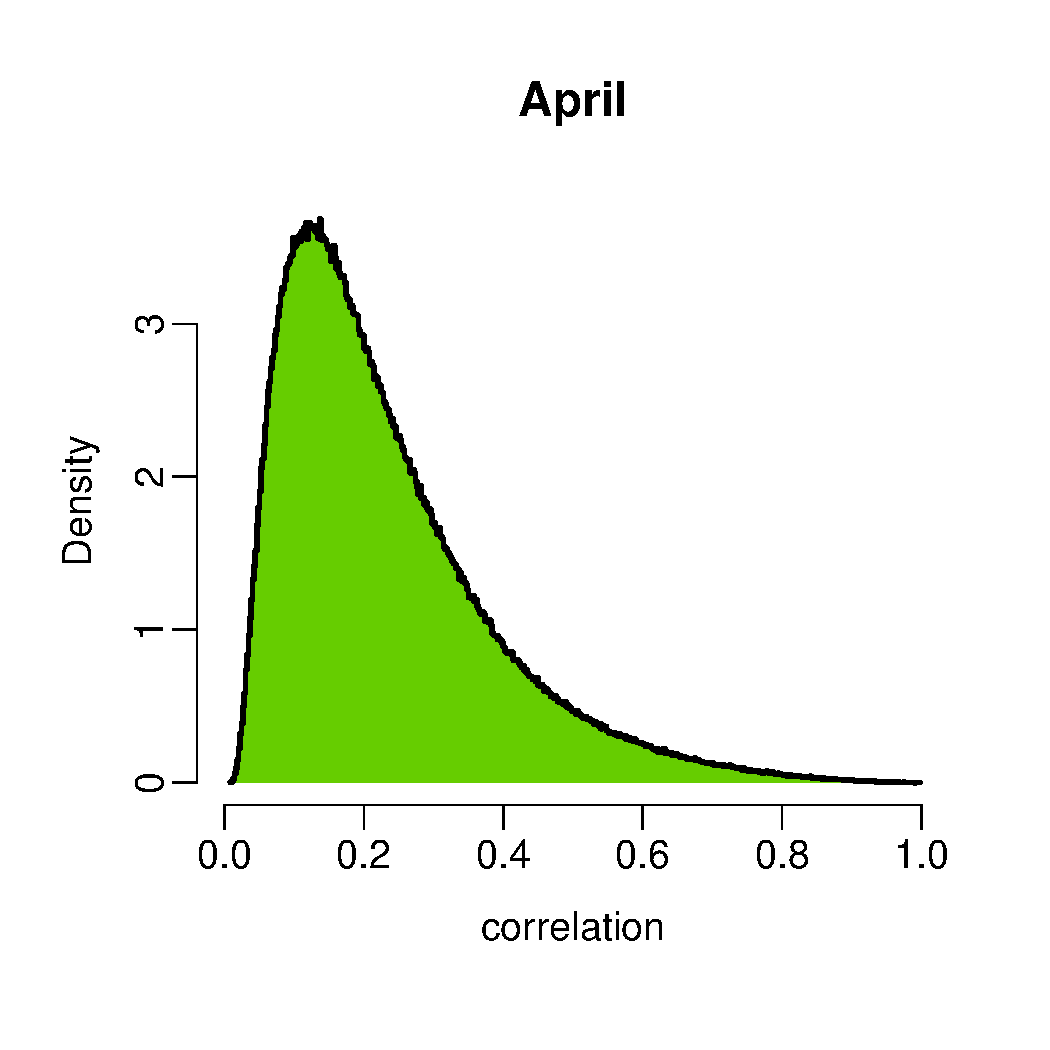
\includegraphics[width=\scale]{Validation_Plots/Correlation/Correlation_04_Apr}\hspace{-1ex}
 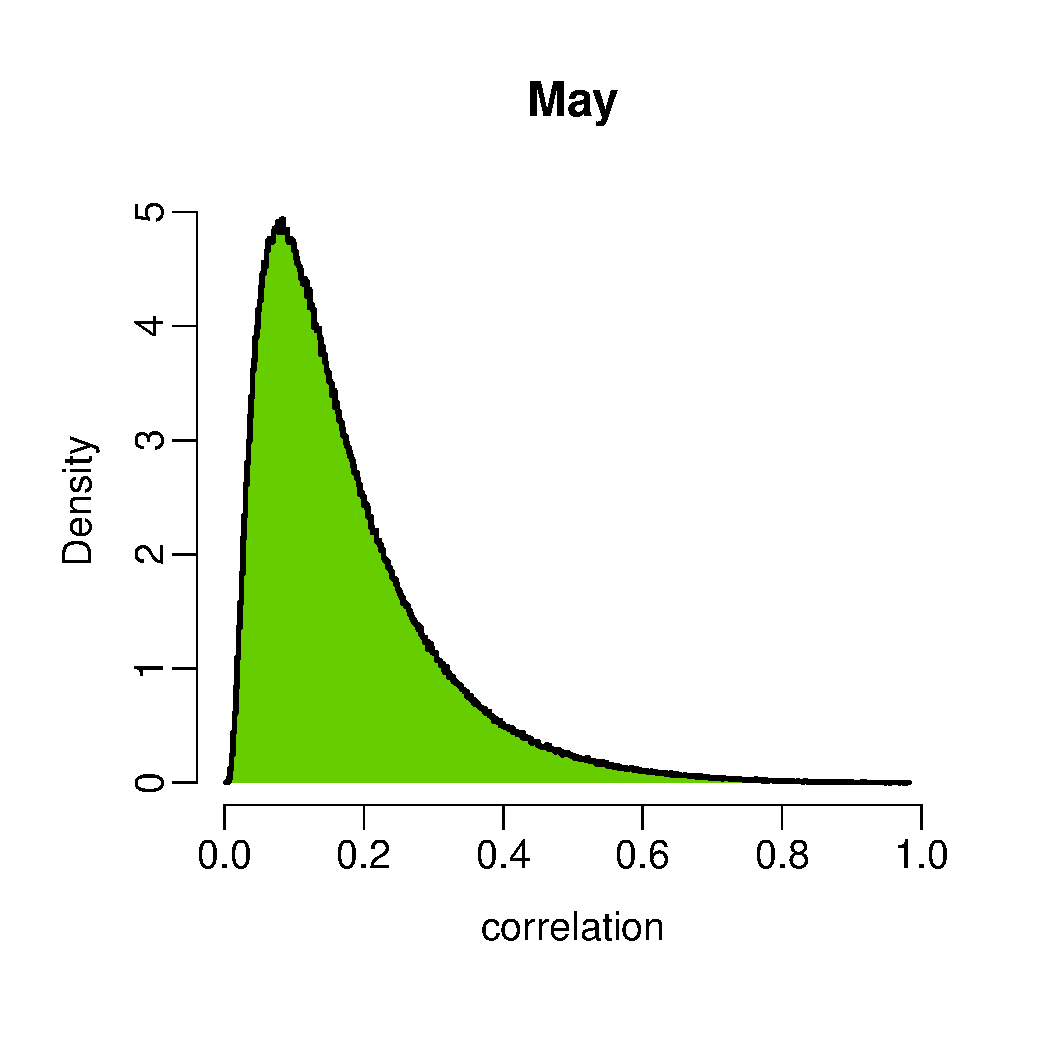
\includegraphics[width=\scale]{Validation_Plots/Correlation/Correlation_05_May}\hspace{-1ex}
 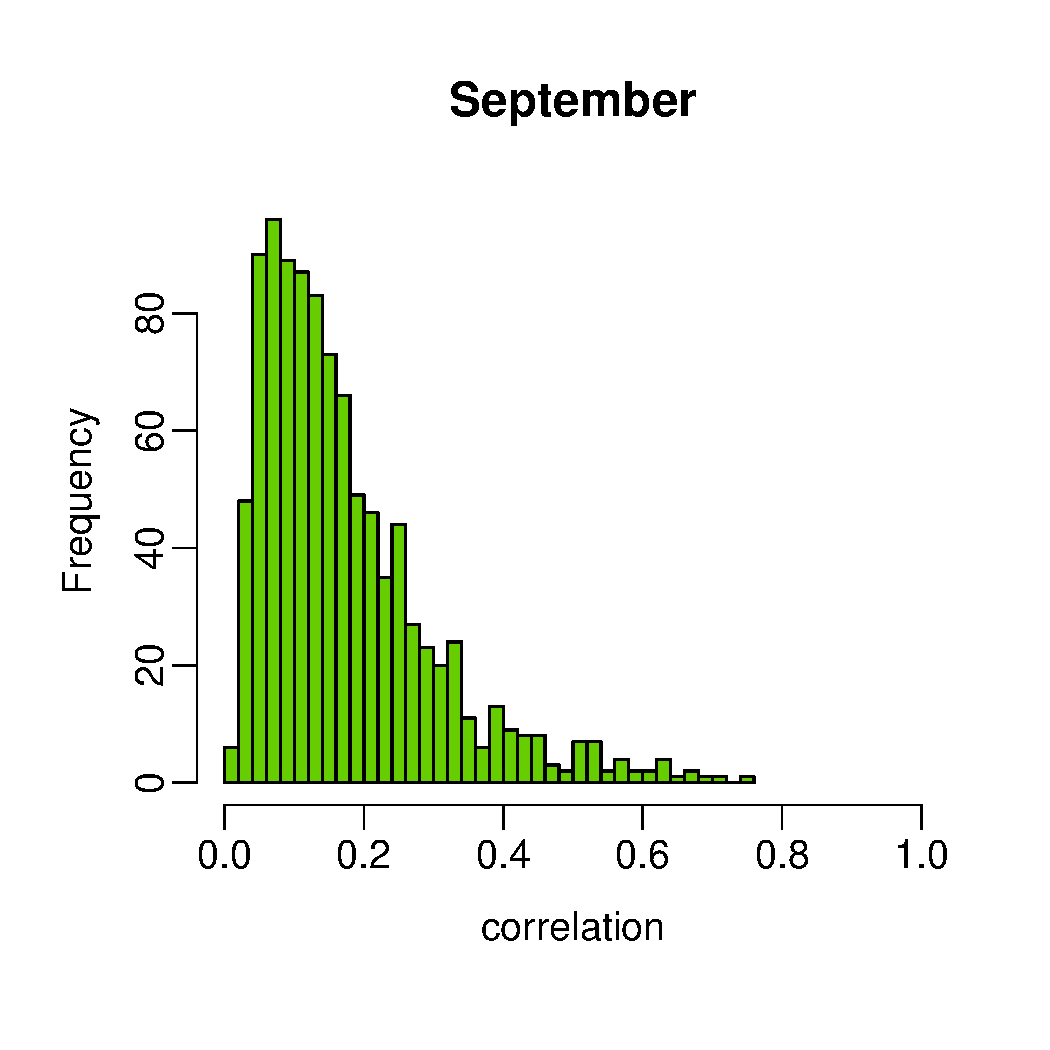
\includegraphics[width=\scale]{Validation_Plots/Correlation/Correlation_09_Sep}\\[-3ex]
 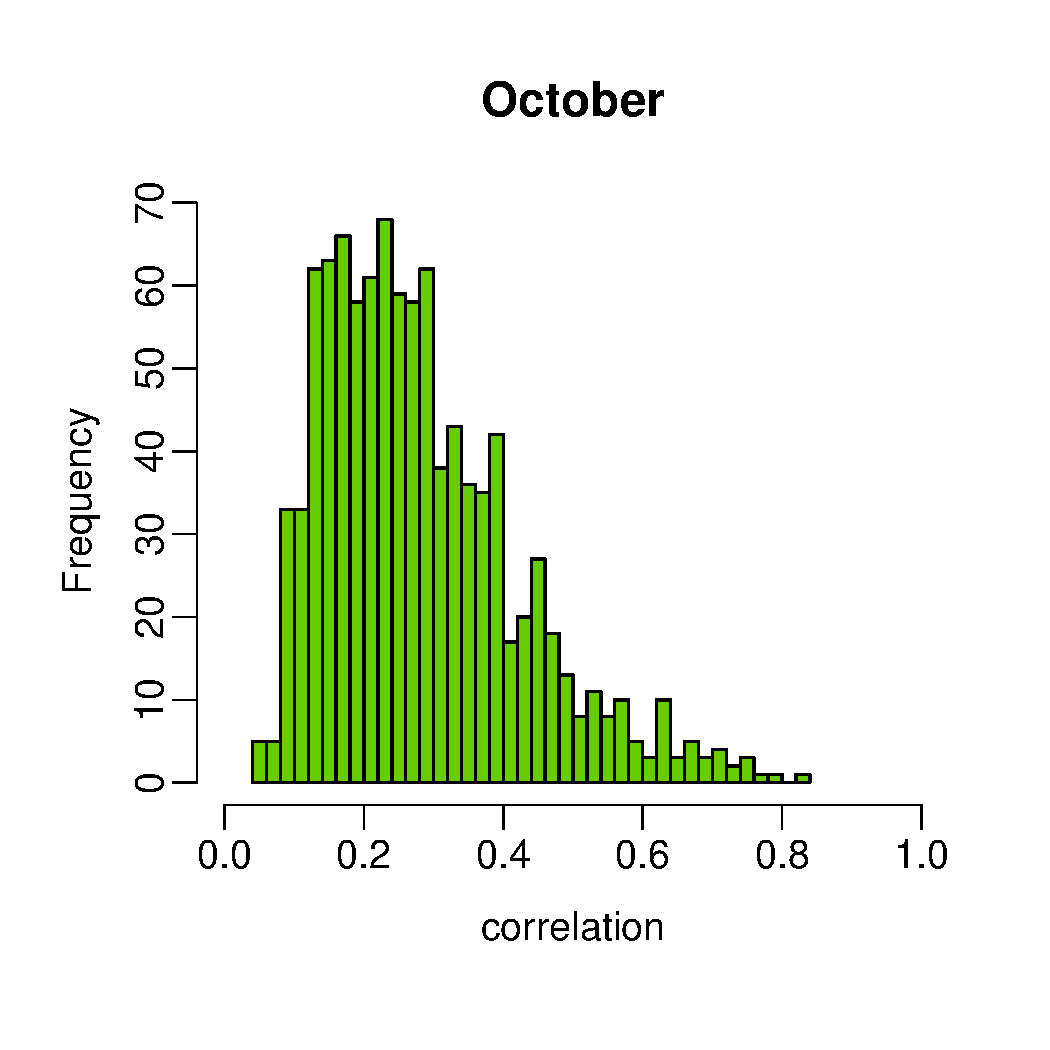
\includegraphics[width=\scale]{Validation_Plots/Correlation/Correlation_10_Oct}\hspace{-1ex}
 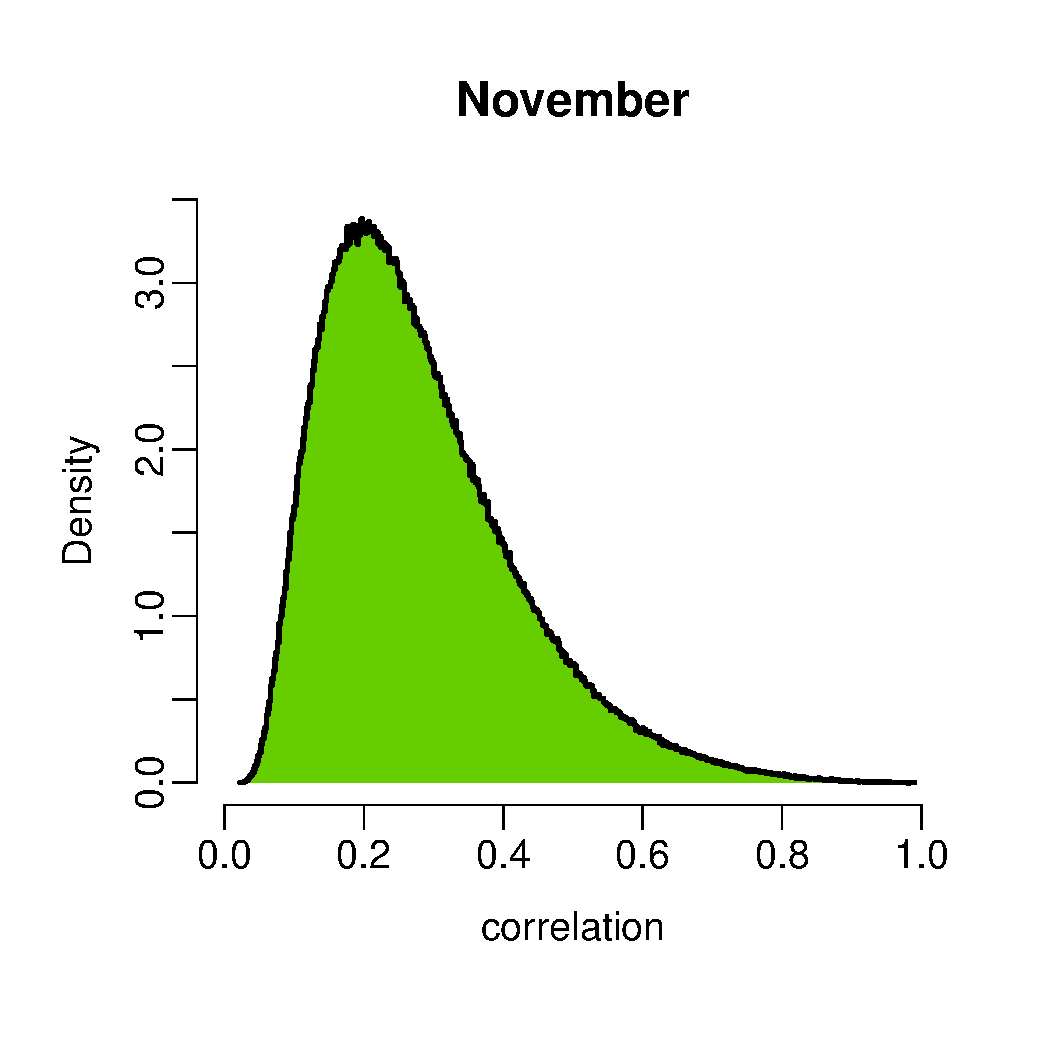
\includegraphics[width=\scale]{Validation_Plots/Correlation/Correlation_11_Nov}\hspace{-1ex}
 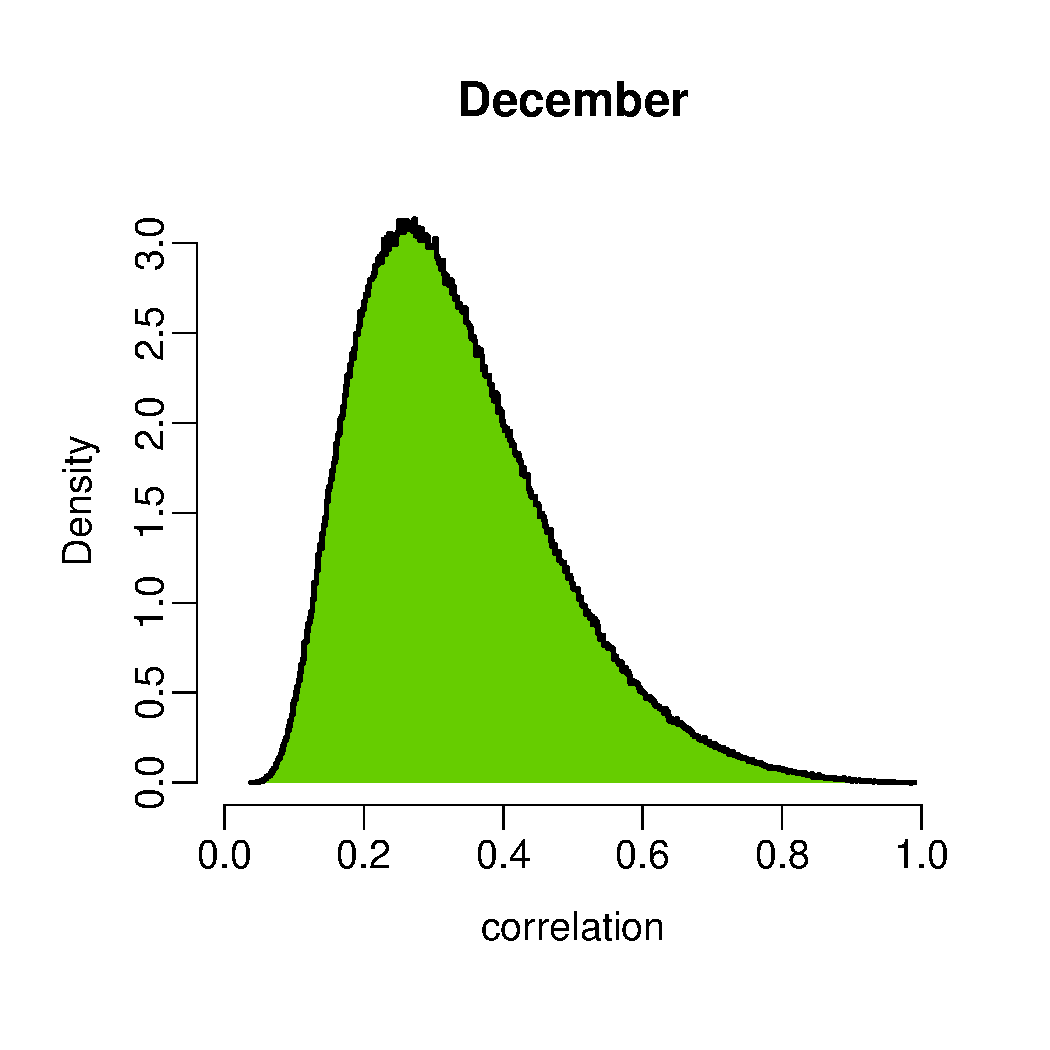
\includegraphics[width=\scale]{Validation_Plots/Correlation/Correlation_12_Dec}
 \caption{Histograms of the correlations between the point at the center of the hypercube $[-1,1]^N$ (where, for each month, $N$ is the number of active inputs) and the 1000 design points.}
 \label{Fig_Correlation}
\end{figure}



\section{Emulators' Validation and Exploration}
This section shows some plots concerning the validation of the previously built emulators. The emulators are validated on the results of 200 simulations not used for training.

\autoref{Fig_Scatter_Errors} shows the standardised errors on the 200 validation point. For each of the 200 points, if $y_i$ is the simulator output, $\hat{y}_i$ the emulator prediction and $\hat{\sigma}_i$ the emulator standard deviation, the standardised error is computed as follows:
\begin{equation}\label{Eqn_St_Er}
\hat{\eps}_i = \frac{y_i - \hat{y}_i}{\hat \sigma_i}.
\end{equation}

\renewcommand{\scale}{12.7em}
\begin{figure}
\centering
 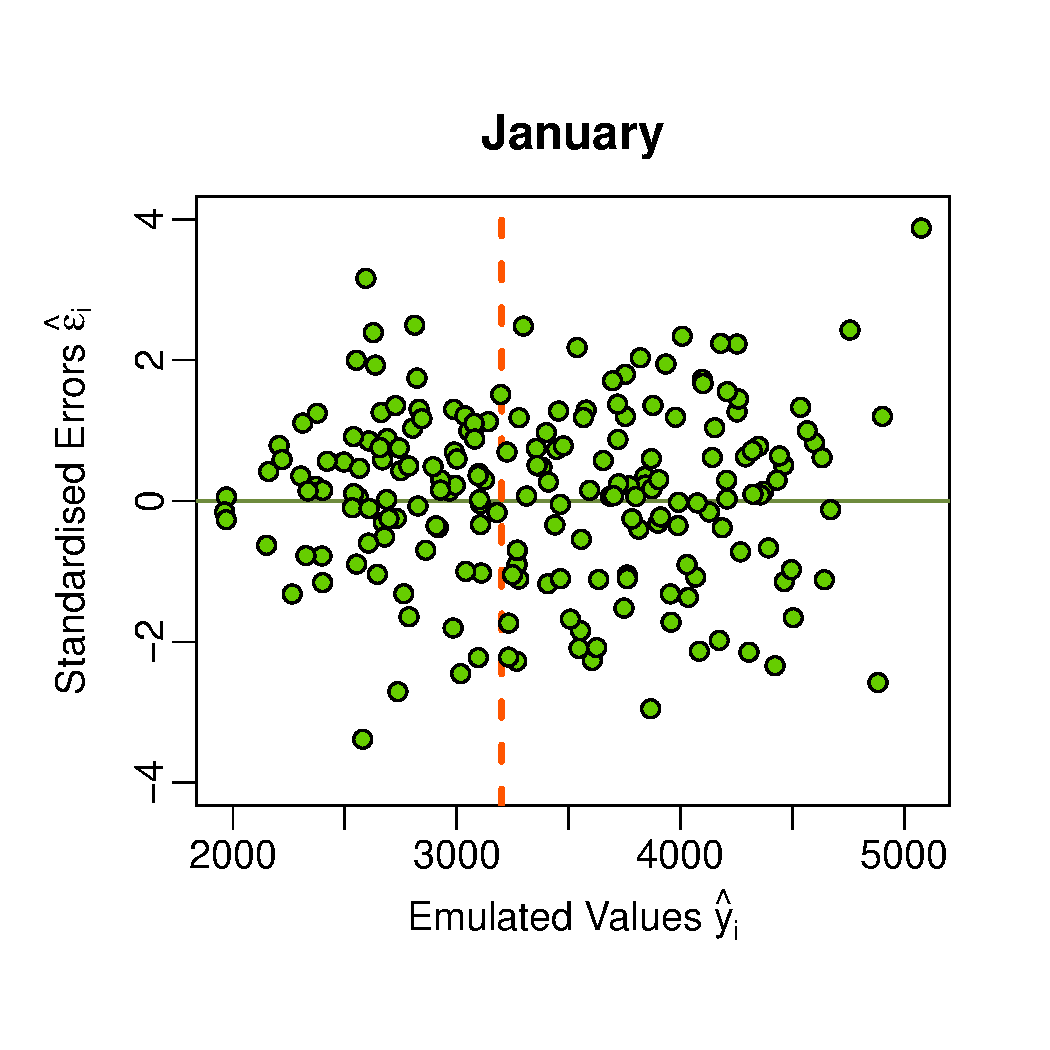
\includegraphics[width=\scale]{Validation_Plots/Validation_Scatter_01_Jan}\hspace{-1ex}
 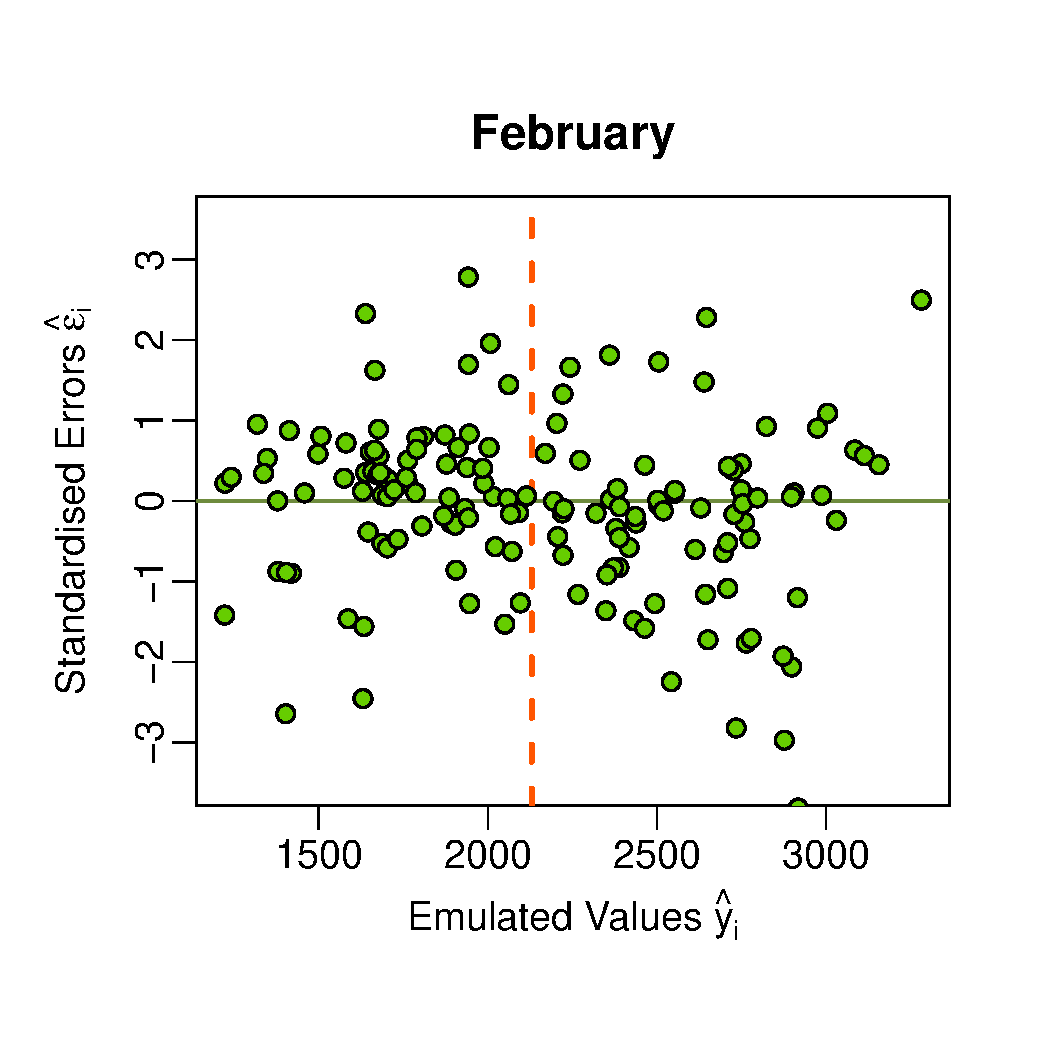
\includegraphics[width=\scale]{Validation_Plots/Validation_Scatter_02_Feb}\hspace{-1ex}
 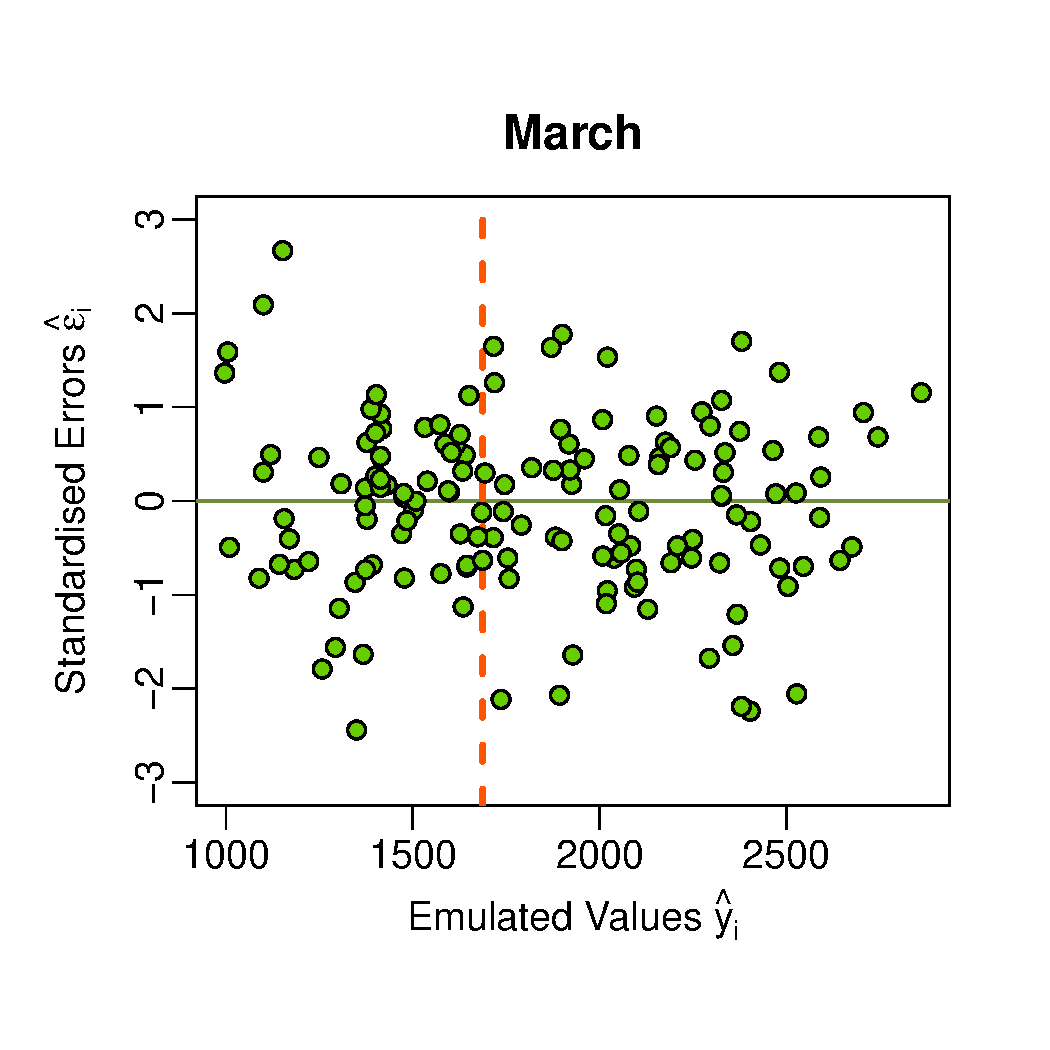
\includegraphics[width=\scale]{Validation_Plots/Validation_Scatter_03_Mar}\\[-3ex]
 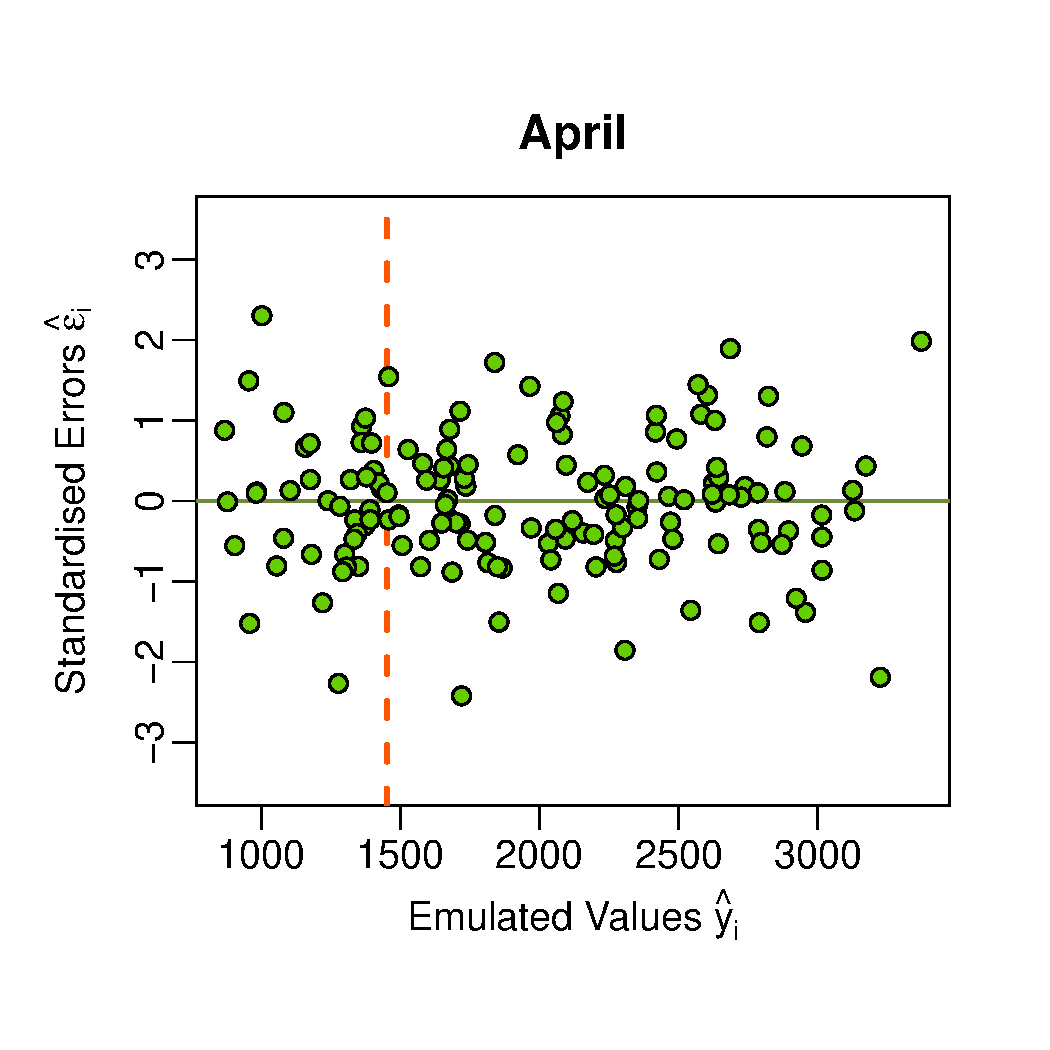
\includegraphics[width=\scale]{Validation_Plots/Validation_Scatter_04_Apr}\hspace{-1ex}
 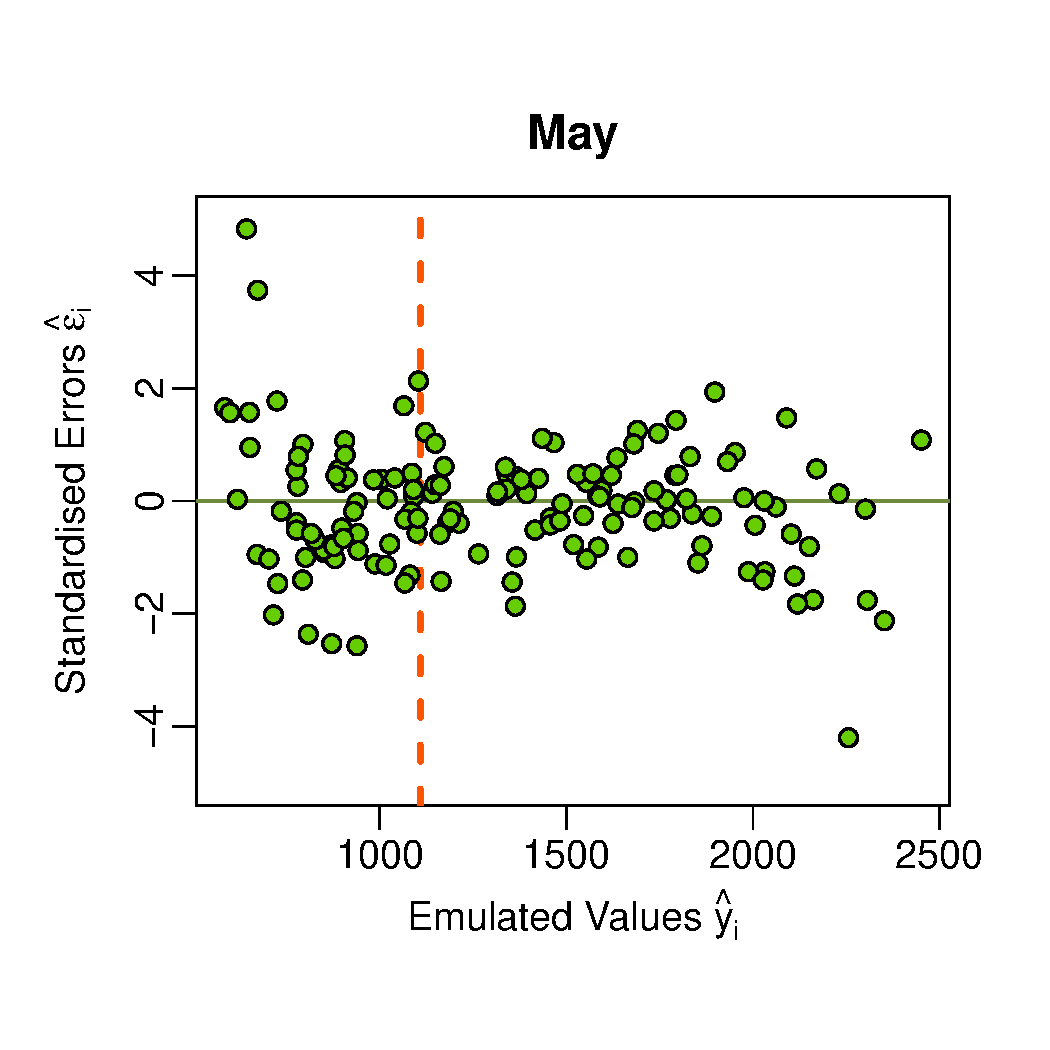
\includegraphics[width=\scale]{Validation_Plots/Validation_Scatter_05_May}\hspace{-1ex}
 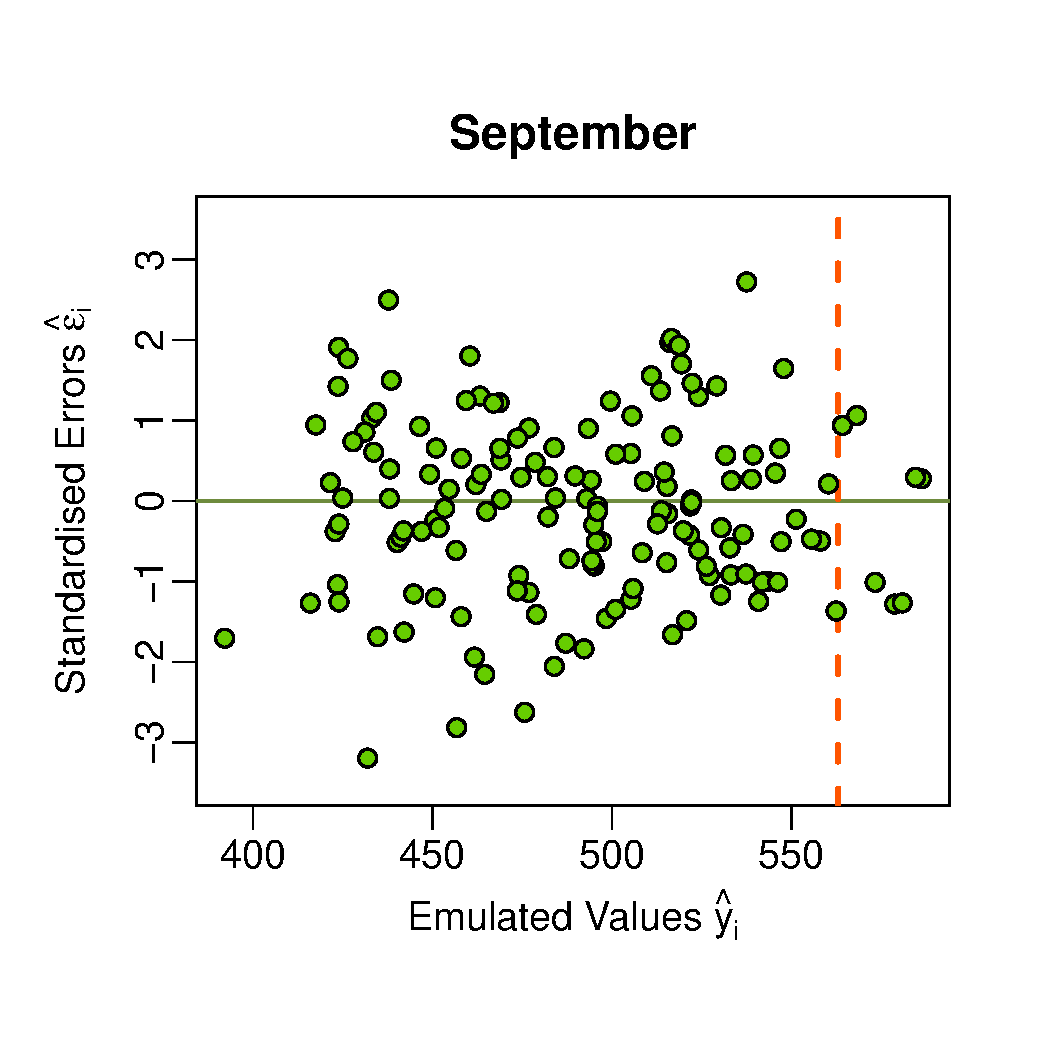
\includegraphics[width=\scale]{Validation_Plots/Validation_Scatter_09_Sep}\\[-3ex]
 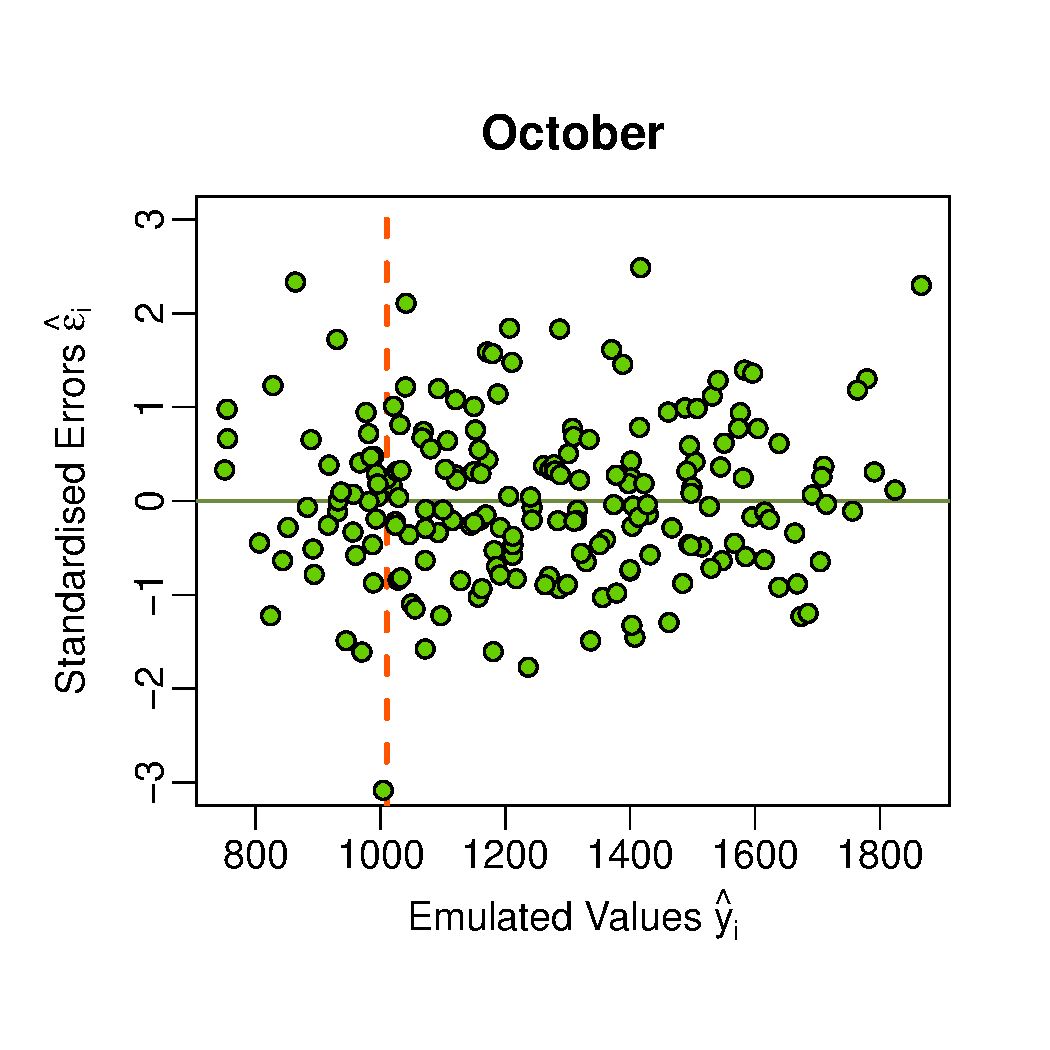
\includegraphics[width=\scale]{Validation_Plots/Validation_Scatter_10_Oct}\hspace{-1ex}
 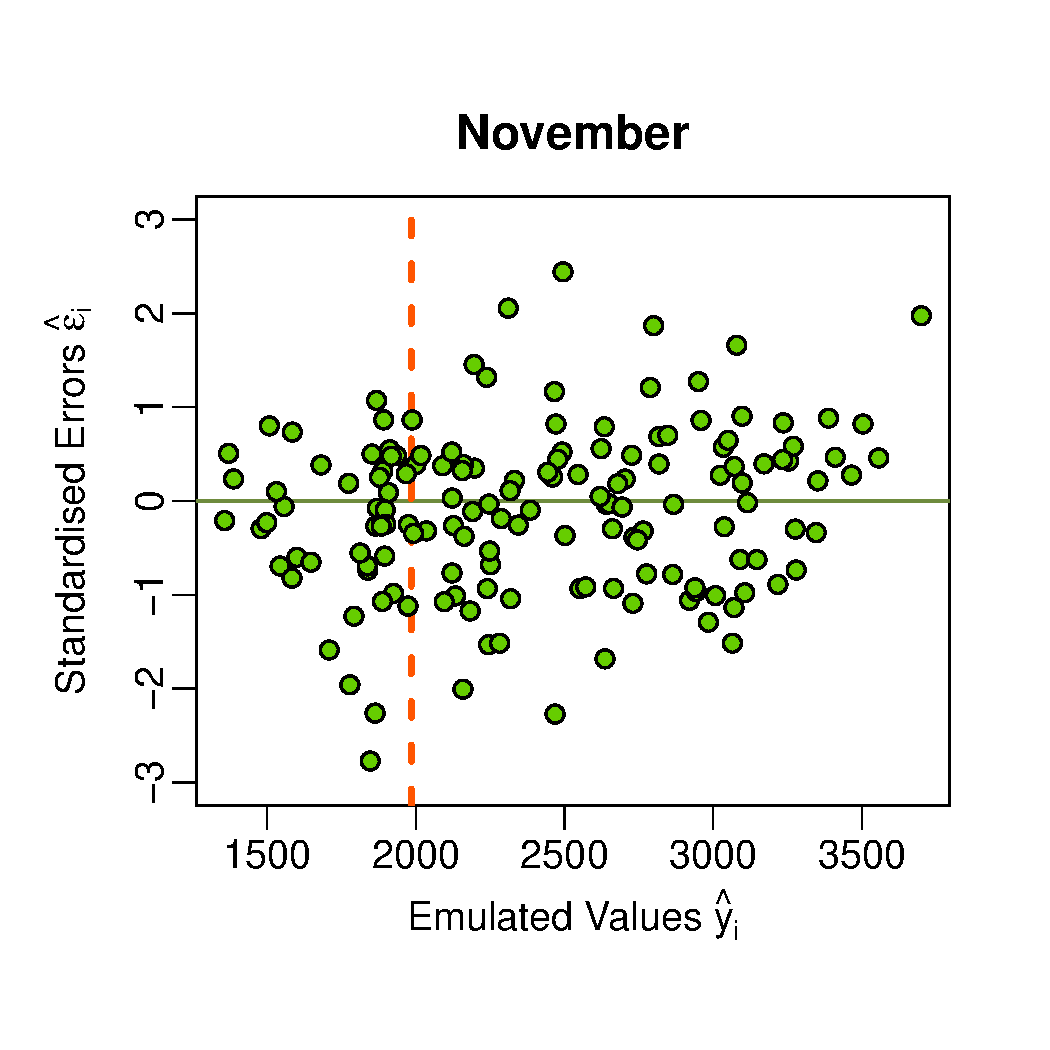
\includegraphics[width=\scale]{Validation_Plots/Validation_Scatter_11_Nov}\hspace{-1ex}
 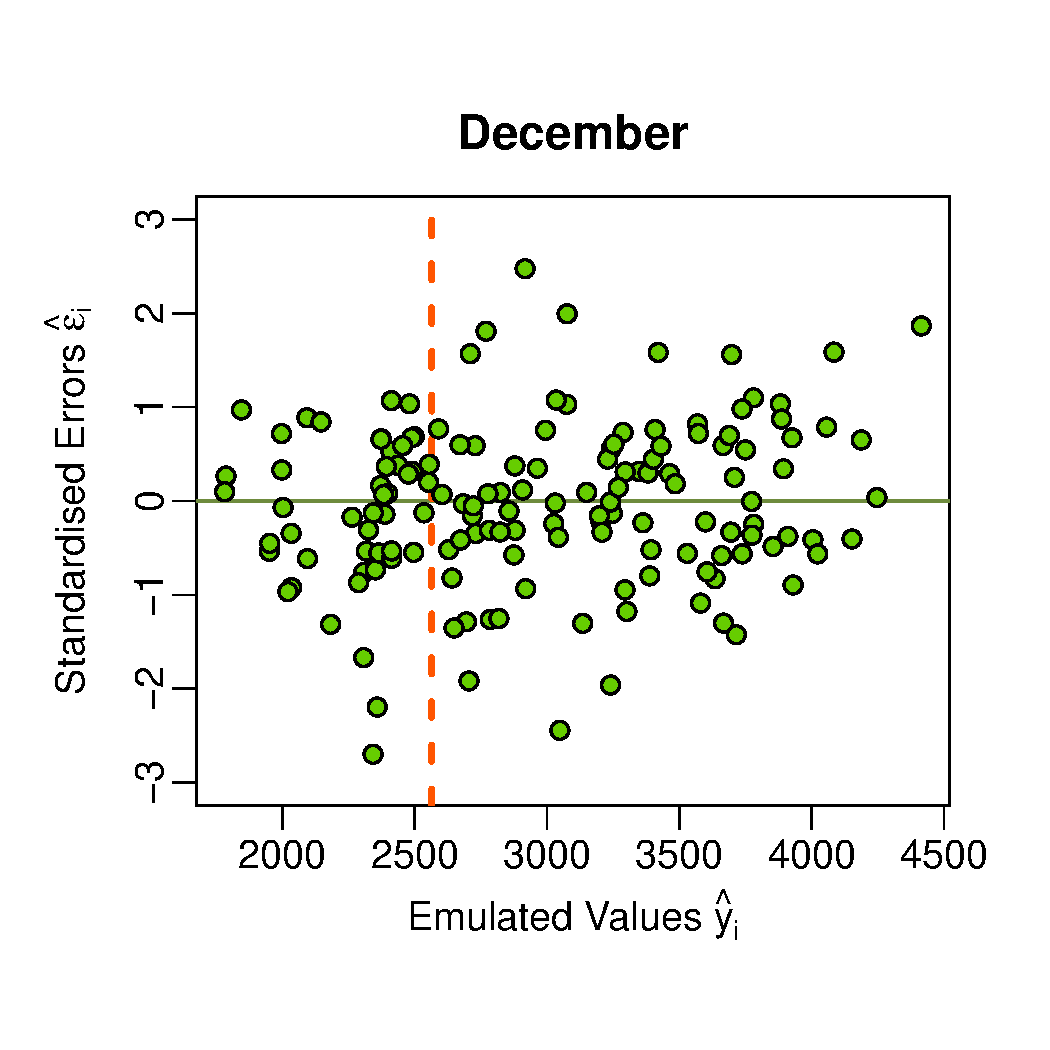
\includegraphics[width=\scale]{Validation_Plots/Validation_Scatter_12_Dec}
 \caption{Validation of the emulators on a set of 200 points. For the different months, the standardised errors in \eqref{Eqn_St_Er} are plotted against the emulator's fitted values. In each plot, the vertical dashed line identifies the value on the $x$-axis corresponding to the observed gas consumption for the month.}
 \label{Fig_Scatter_Errors}
\end{figure}


\subsection{Comparison Between LR and Trained Emulators}

For each month, \autoref{Table_sigma} compares the prior variance of the emulator (\ie, the variance of the original linear regression residuals) with the adjusted variance of the emulator predictions on the 200 validation points. I am reporting the $2.5$ and $97.5$ empirical percentiles of these, to get a sense of the difference in prediction uncertainty between the original linear regression and the trained emulators.

\begin{table}
 \centering
 \renewcommand{\arraystretch}{1.4}
 \newcommand{\colsep}{3ex}
 \caption{For each month: the first line of the table shows the variance of the linear regression residuals (prior cumulative variance of the emulator). The second and third lines show the $2.5$ and $97.5$ empirical percentiles of the emulator variances at the 200 validation points.}
 \begin{tabular}{c<{\hspace{\colsep}}ccccccccc}
\specialrule{.1em}{0em}{0.1em} 
 &  \textbf{Jan} & \textbf{Feb} & \textbf{Mar} & \textbf{Apr} & \textbf{May} & \textbf{Sep} & \textbf{Oct} & \textbf{Nov} & \textbf{Dec}\\
 \specialrule{.05em}{.1em}{0.1em} 
 \specialrule{.05em}{0em}{0.2em} 
  $\sigma^2$  & 84.86 &  50.63  &  49.14  &  49.58  & 206.70  &  0.88 &  23.20 & 57.22 &  67.65\\
  $[2.5\%$,       & 6.4      & 10.6     &  3.2      & 4.5        & 13.3      & 0.07  & 1.51    & 3.7      & 4.17\\
  $97.5\%]$ CI & 29.1    & 43.4     & 11.5     & 22.6     & 53.8      &  0.35  & 5.41    & 13.35  & 12.67\\
 \specialrule{.1em}{0.2em}{1em} 
 \end{tabular}
\label{Table_sigma}
\end{table}

Finally, \autoref{Fig_Comparison_LR} allows to compare graphically the accuracy of the emulator's predictions versus the linear regression's ones. The plot concerns the month of March, and only results for 10 of the 200 validation points are shown (10 consecutive ones in terms of the simulator outputs), to avoid cluttering which would prevent details to be appreciated. 

The red ``cat's eye'' boxes represent the emulator predictions for these points, within a range of three standard deviations from the mean prediction. The blue star and the yellow squares represent instead the real simulator outputs and the linear regression predictions, respectively. It can be appreciated that the emulator is often much more precise than the linear model, and has a high level of confidence in its prediction (small uncertainty bands).




\begin{figure}
\centering
 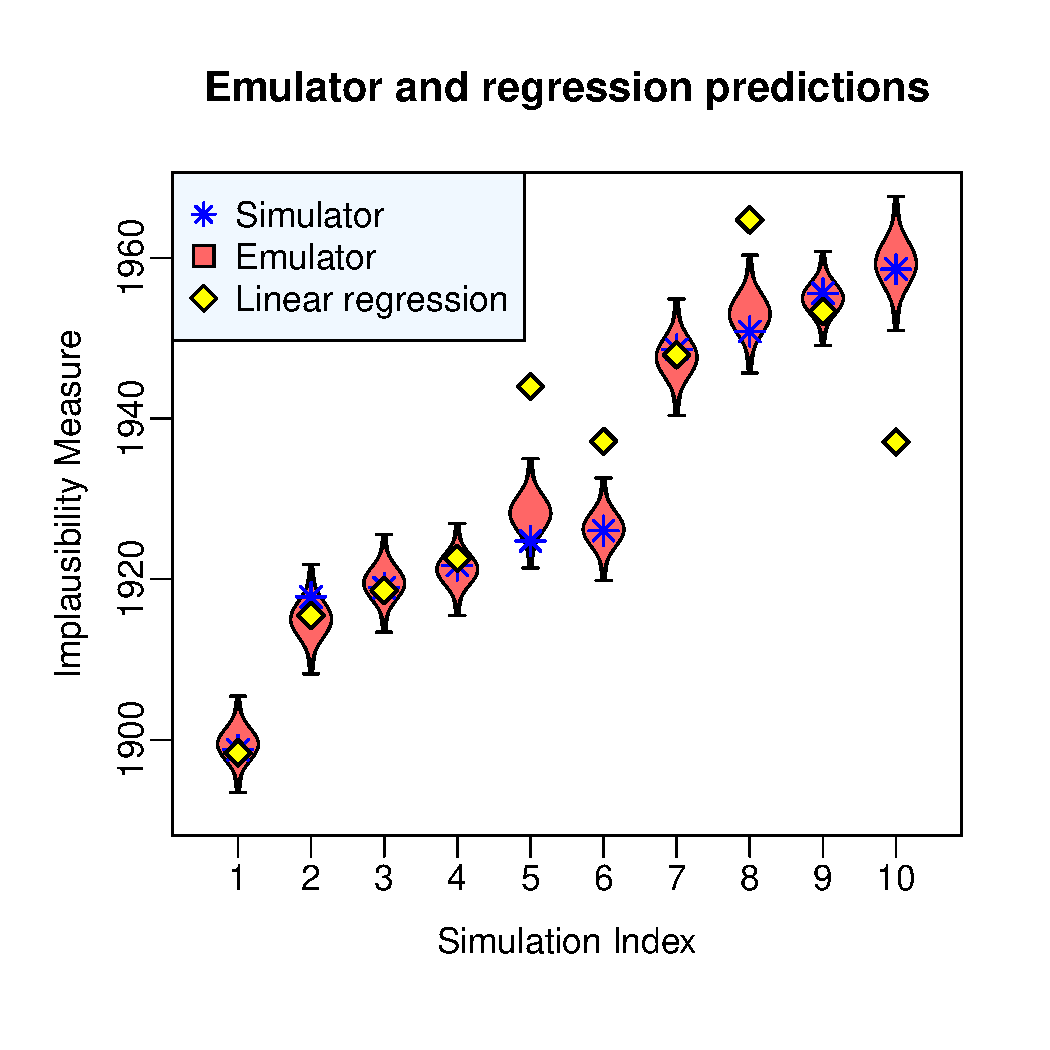
\includegraphics[width=0.8\textwidth]{Validation_Plots/Comparison_LR/LR_Mar_111-120}
 \caption{Visual comparison between emulator (red cat's eye boxes) and linear regression (yellow squares) predictions. The plot concerns 10 validation points of the month of March. The height of the emulator cat's eye boxes cover a range of three standard deviations from the emulator's mean prediction.}
 \label{Fig_Comparison_LR}
\end{figure}







\end{document}
